% 5) Methods - provide a description of the way in which you intend to address the research question.  This means describing the existing tools/systems that you will use, new tools or systems that you will build and the experiments that you will conduct.
\section{Results}
\subsection{Harpocrates}
We designed a system, Harpocrates (Greek god of silence, secrets, and confidentidality), which allows users to easily compensate publishers at a fair rate for their content.
Harpocrates is composed of a client-side browser extension for users and a server for accounting.
Furthermore, it fits into the current ad ecosystem with minimal implementation work required for publishers.

\subsubsection{Design Considerations}
In designing Harpocrates, there was a clear set of requirements whic, if not accomplished, would yield a system infeasible for wide deployment.
First, it must address the needs of current ad-blocker users, else they would not consider using it.

It must also be unobtrusive and get our of the user's way.
For example, with our current design, there is a very simple settings page that allows the user to pick a budget, etc.
The rest of the logic happens erver-side, improving user experience.

Performance must improve over the current Web experience without an ad-blocker.
Surveys show that a substantial proportion of users use ad-blockers for performance reasons~\cite{hubspot2016adblock}, so any substitute should strive to address that concern specifically.

The system should fit into the current Web ecosystem, i.e. must not rely on any new standards in order for it to see wide adoption.
Correspondingly, the implementation cost for publishers must be minimized, because it will never see wide adoption without publishers' acceptance.
This means that solutions that involve adding server-side code, such as would be required to enable many of the services described in Section ~\ref{academic_related}.

Finally, it must provide control over the browsing experience for both users and publishers alike.
Currently, publishers are essentially locked in to using a combination of subscription and ad tactics for revenue.
By enabling them to recoup some of the lost revenue due to blockers, and enabling users to opt-in to funding their favorite content, both parties benefit.

\subsubsection{Architecture}
Our solution relies on fact that ad exchanges are efficient marketplaces for determining the fair value for a given piece of real estate on the internet.
In order to take advantage of this fact, Harpocrates sits inline in the ``waterfall'' (Figure ~\ref{fig:waterfall}).

\begin{figure}[h]
\centering
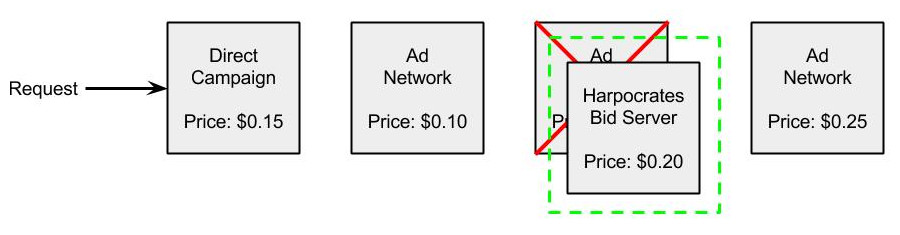
\includegraphics[width=0.5\textwidth]{waterfall}
\caption{Harpocrates sits inline with the current ad exchange ecosystem.}
\label{fig:waterfall}
\end{figure}

From the publisher's point of view, Harpocrates is essentially another ad network, which, given an impression, returns a bid for the ad (or none).
Hence, its implementation cost is no higher than that of adding another ad network for a given publisher.

From the user's point of view, Harpocrates is simply a browser extension.
Given a number of initial settings (Figure ~\ref{fig:harpocrates_ui}), Harpocrates will make bids on the user's behalf for a given ad.

\begin{figure}[h]
\centering
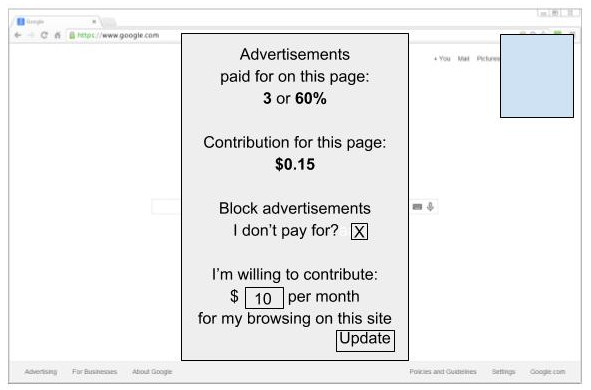
\includegraphics[width=0.5\textwidth]{harpocrates_ui}
\caption{For the user, Harpocrates simply requires installing a browser extension and initializing a few settings.}
\label{fig:harpocrates_ui}
\end{figure}

Finally, Harpocrates also acts as a clearinghouse, settling account monthly.
for a given set of publishers $N$ and users $M$, only $O(|N| + |M|)$ payments need to be transacted (i.e. one payment from each user to Harpocrates, and one payment from Harpocrates to each publisher).
At scale, we gain a lot from this aggregation of payments when compared to a system such as paywalls, which requires $O(|N| \cdot |M|)$ payments (one for each user/publisher pair) in the worst case.

These aspects of the architecture make Harpocrates a good candidate solution, given the aforementioned design considerations.
It addresses the needs of current ad-blocker users by showing them fewer ads, the user interface makes it practically invisible from a user's point of view, and performance is improved by eliminating the actual delivery of ad media content (Figure ~\ref{fig:harpocrates}).
Harpocrates also fits into the current complex ecosystem, requiring no new standards.
Finally, the implementation is simply adding another ad network, minimizing implementation costs.

\begin{figure}[h]
\centering
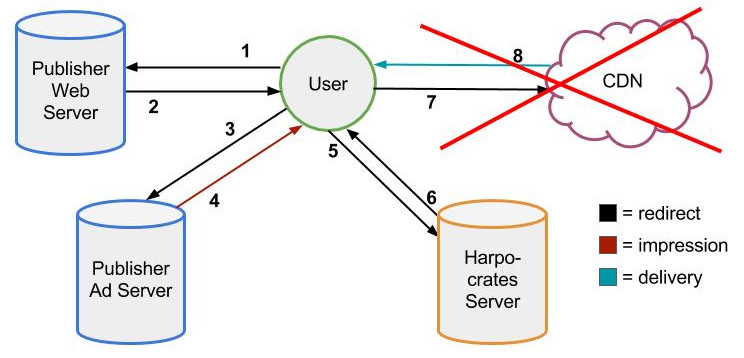
\includegraphics[width=0.5\textwidth]{harpocrates}
\caption{Harpocrates removes the actual ad media element delivery process, cutting out a roundtrip request to the ad server content delivery network and improving performance.}
\label{fig:harpocrates}
\end{figure}

\subsection{\textit{Un}acceptable Ads}
\textit{Un}acceptable Ads is a proof of concept to illustrate a more immediate path forwards for users who block ads because of the reduced performance and/or visual obtrusiveness.
Relying on the idea that users are willing to see some ads in order to support content publishers, our goal is to allow users to specify the number and type of ads that they don't want to see.
This idea is similar in motivation to the Acceptable Ads program run by Adblock Plus, but where Acceptable Ads are determined by the Adblock Plus organization and advertisers can pay to be whitelisted, our system will put the control directly in the user's hands.
To realize this idea, we have modified two Chrome extensions: uBlock Origin, a request-based blocker, and a ``perceptual blocker'' which was recently developed by Storey, et al.~\cite{storey2016future} at Princeton University.

\subsubsection{uBlock Origin}
uBlock Origin is a popular open source desktop ad-blocker with nearly 9 million installs on Google Chrome as of May 2017.
This blocker is categorized as a request-based blocker, meaning that it recognizes web requests which are targeted at ad-related servers and prevents them from ever leaving the client's browser.
This strategy offers significant performance benefits, as it reduces network traffic and prevents (often large) media elements from being received and rendered in the client browser.
Identifying ad-related network requests is done by matching target URLs against a list of known advertising URLs (e.g. EasyList~\cite{easylist}).
The extension uses multiple such community-maintained lists, and matches against them using a combination of simple lookups and regular expressions.

Our modification to the uBlock Origin is a notion of ``Ad Tolerance'', a configurable setting from 0-100\% which determines what proportion of ads will be shown to the user on any given page.
If the user has their tolerance set to 0\%, the extension will block all ads like uBlock Origin usually does and if the user has their tolerance set to 100\% then the extension won't function as an ad-blocker at all.
Any setting between 0 and 100\% will result in each ad element probabalistically being blocked.
The reason for probabalistic blocking is that it is a very difficult problem to predict the number of total ads that will be shown on a page before the page has fully rendered, so blocking a pre-determined number of elements is impractical.
While probabalistic dropping means that the proportion of ads blocked might not be exactly as expected on every page, in the long run the number of ads blocked will very closely match the specified proportion.

\subsubsection{Perceptual Blocker}
Storey, et al.~\cite{storey2016future} recently published work on what they dubbed a ``perceptual blocker'', which blocks ads based on their visual content rather than their associated web requests or the structure of the page.
The primary observation which this work is based on is that there have been many efforts recently to standardize ad policies on the internet through joint coalitions such as AdChoices~\cite{adchoices}.
Such programs require ads to identify themselves by including text such as "from our advertisers" or by displaying a common logo, such as the AdChoices logo.
Storey, et al. recognize that this offers an opportunity to visually recognize and identify ads as a human would be able to.
The blocker that they developed puts this idea into practice, and covers all visually recognized ads with a banner reading "THIS IS AN AD."
Covering ads rather than completely hiding them is deliberate, as the researchers wanted to avoid potential backlash from the advertiser community, who are discomforted by the idea that their ads could be completely delivered but still not presented to a user - leaving them paying for an impression which didn't actually happen.
This raises a broader question about the morality of perceptual blockers, and suggests that if these blockers were to become popular, advertisers would have to make a significant engineering effort to maintain accurate impression accounting in their presence.

Our first modification to the perceptual blocker is the same as that which we made to uBlock Origin, adding a configurable tolerance level which probabalistically blocks the ads it encounters.
We also added a second configuration to this blocker, which allows the user to specify a maximum width and height of ad elements which they are willing to see (Figure ~\ref{fig:unacceptable_ui}).
This highlights a key benefit to the perceptual blocker, because the ads are completely delivered before blocking occurs, the blocker has a more complete set of information about the ad's qualities (e.g., size, content, placement on the page) when the blocking decision is made.
We use this additional information to block ads above a certain size, but this could be extended to other configurations, such as even recognizing and blocking inappropriate ads.

\begin{figure}[h]
\centering
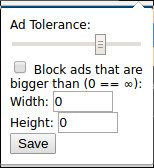
\includegraphics[width=0.15\textwidth]{unacceptable_ui}
\caption{User interface for our modification of the Perceptual Blocker.}
\label{fig:unacceptable_ui}
\end{figure}

\begin{figure}[h]
\hfill
\subfigure{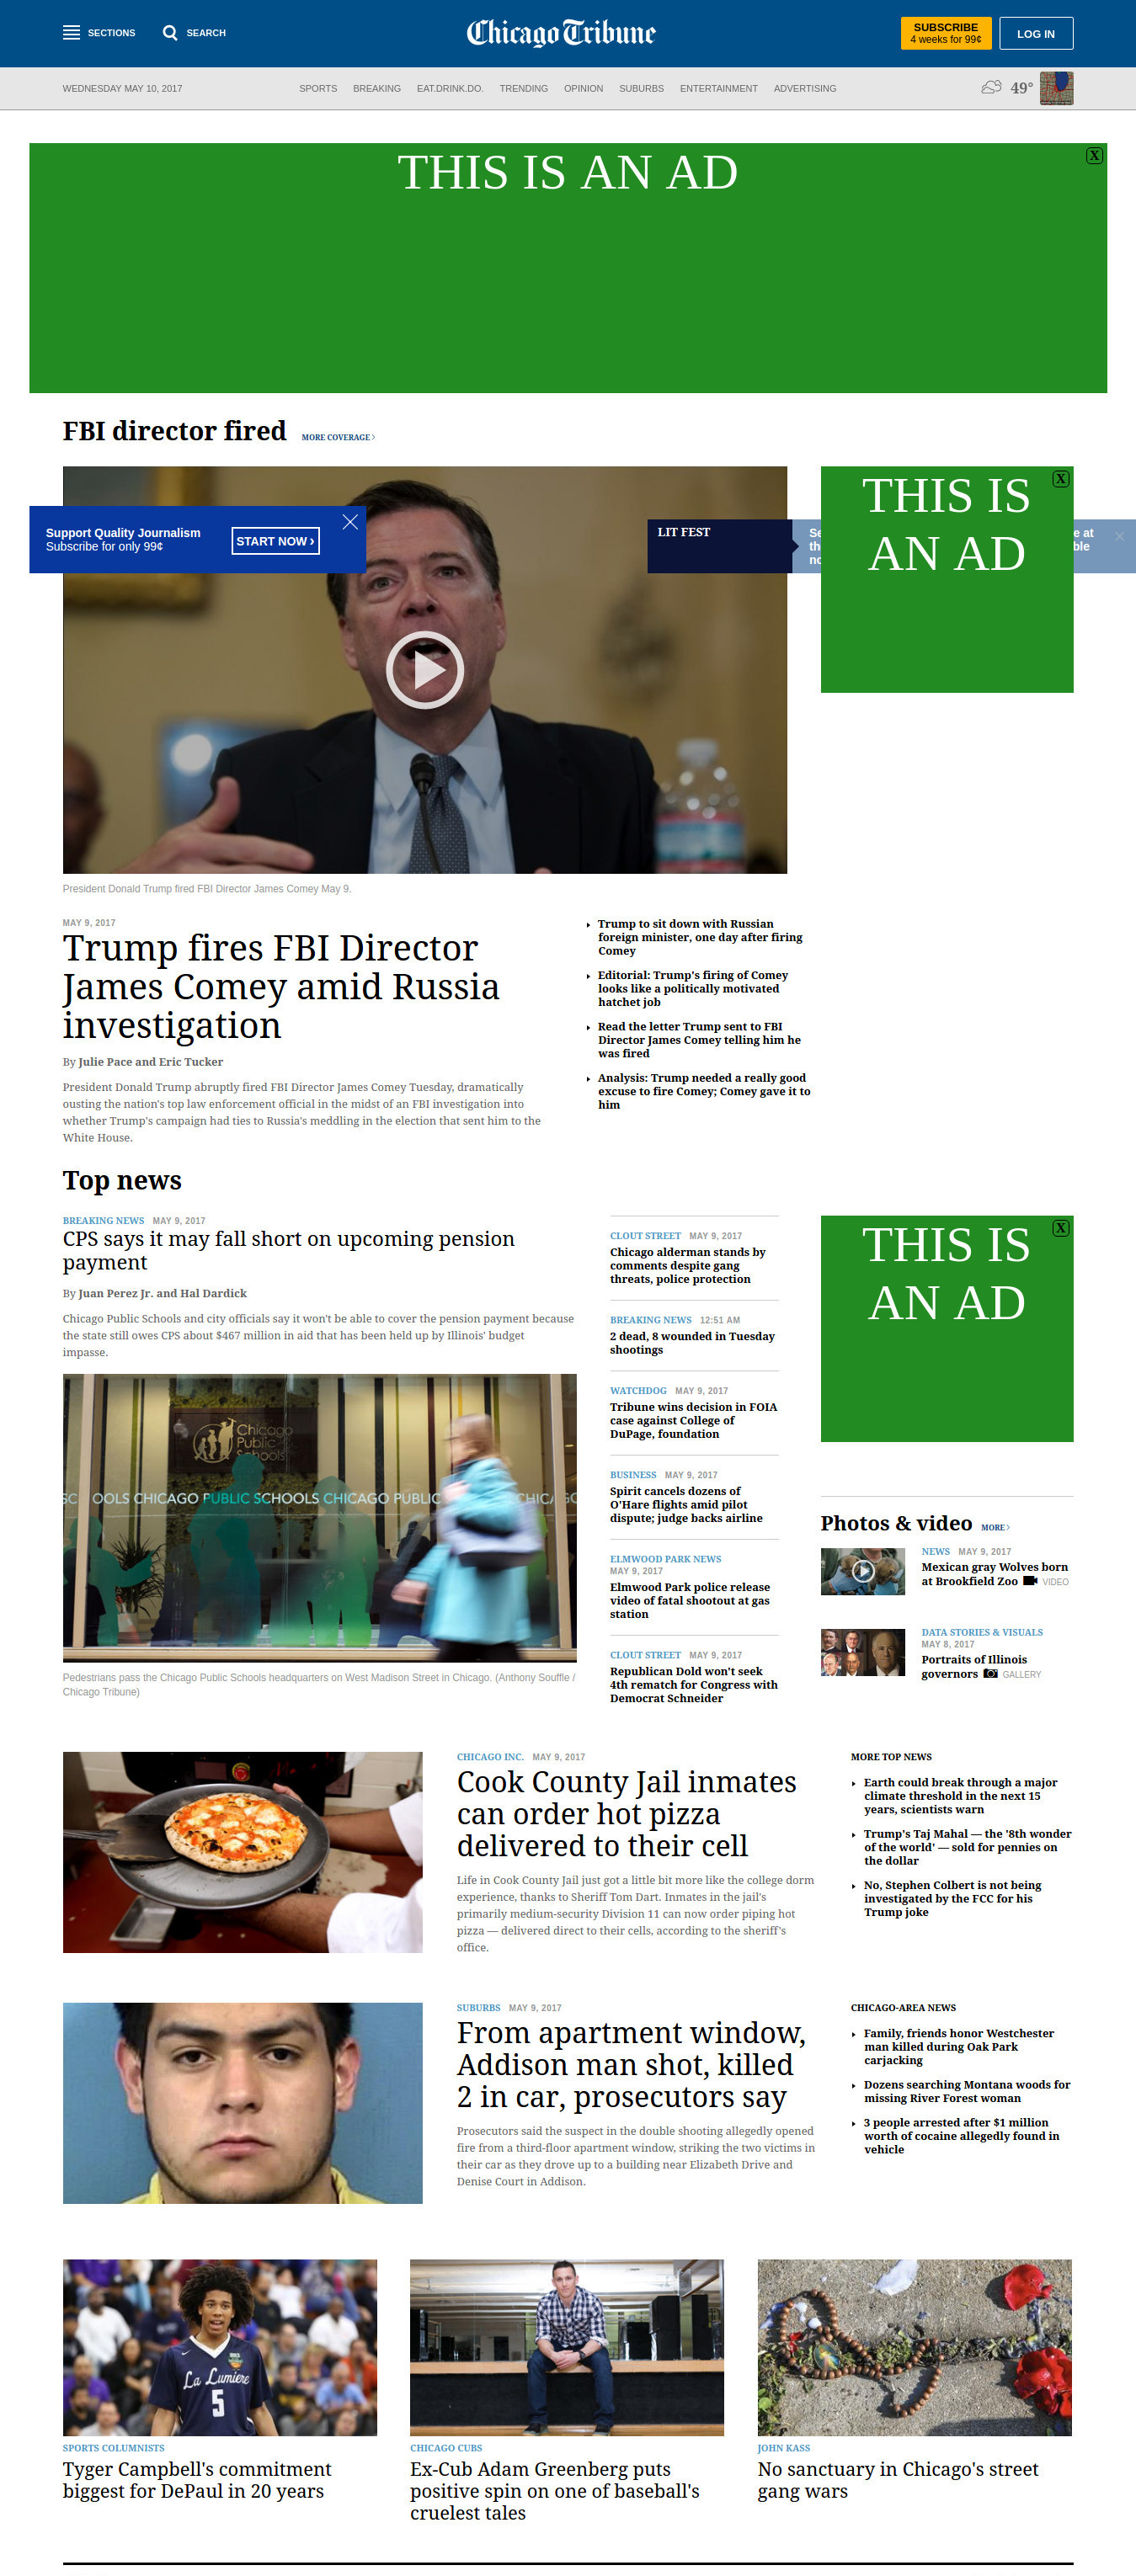
\includegraphics[width=0.15\textwidth]{unacceptable_no_tolerance}}
\hfill
\subfigure{
\includegraphics[width=0.15\textwidth]{unacceptable_high_tolerance}}
\hfill
\caption{\textit{Un}acceptable Ads allows the user to select their tolerance for advertisements, from 0\% (left) upwards (right).}
\label{fig:unacceptable}
\end{figure}

\subsection{Performance}
In order to assess the impact of ad-blockers on performance, we performed an experiment to measure page load times with and without uBlock Origin enabled.
The five sites which we chose to measure load times on were the five most popular news sites based on the Alexa ranking~\cite{alexa}
We loaded each site 10 times under each condition and averaged the results, closing the browser between loads to ensure that a full rendering occured.
Page load times were measured using the Chrome extension "Page Load Time~\cite{pageloadtime}, which considers a page fully loaded once all elements have finished rendering.
We deliberately chose not to clear the local browser cache between page loads, recognizing that in practice web content is often cached locally.
The results backed up survey findings that many users use ad-blockers for performance reasons~\cite{hubspot2016adblock}, as there was a 2.33x speedup with uBlock enabled (Figure ~\ref{fig:load_times}).

\begin{figure}[h]
\centering
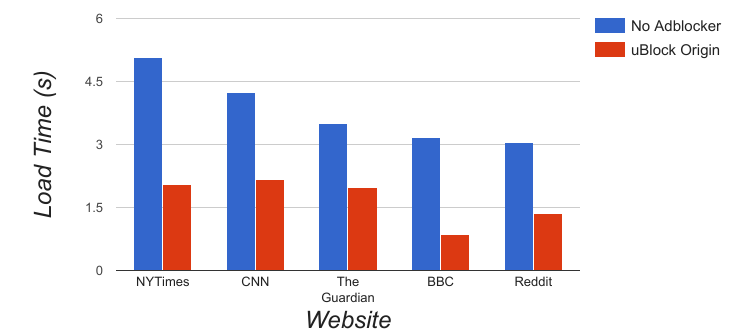
\includegraphics[width=0.5\textwidth]{load_times}
\caption{Loading times for five popular websites with and without the popular ad-blocker uBlock Origin.}
\label{fig:load_times}
\end{figure}

To assess the performance of our \textit{Un}acceptable Ads extensions, we performed a similar experiment by measuring page load times for the Chicago Tribune homepage at multiple different levels of ad tolerance.
Our findings are consistent with our intuition: since uBlock Origin blocks based on network requests, performance should decrease as tolerance goes up.
For the Perceptual Blocker, however, performance stays relatively constant regardless of tolerance, since ads are detected and hidden after they are loaded (Figure ~\ref{fig:load_times_over_range}).
This difference highlights the key benefit to request-based blockers: performance.
Preventing web requests from ever leaving the client browser results in a decrease in network traffic and the costly rendering of media elements.
One thing to note is that we consider a page to be done loading when the page is fully rendered, but this doesn't include the additional time required in the case of the perceptual blocker to identify and cover ads.
While this occurs quickly, there is some computational overhead associated with visually scanning the web page which should be considered when comparing the two techniques.

\begin{figure}[h]
\centering
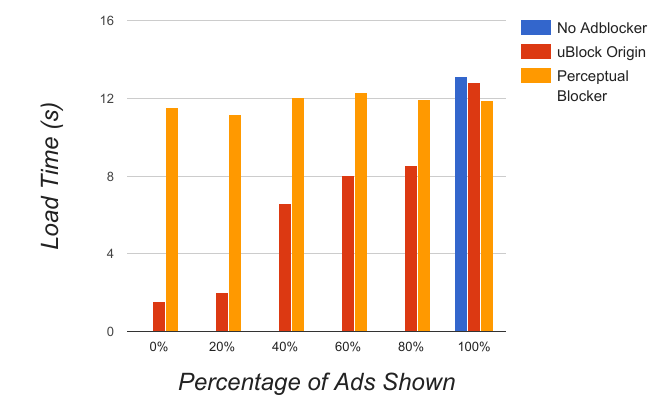
\includegraphics[width=0.5\textwidth]{load_times_over_range}
\caption{Loading times for Chicago Tribune homepage with varying levels of tolerance for ads using the \textit{Un}acceptable Ads extension (``Perceptual Blocker'') and a modified version of uBlock Origin.}
\label{fig:load_times_over_range}
\end{figure}

\subsubsection{Summary and Technical Challenges}
These extensions serve as two separate proofs of concept for a new generation of ad-blockers which could allow for a more fine-grained tuning of what types of ads are blocked.
This approach can provide partial or full compensation for the publisher while still addressing user concerns about the performance and/or visual issues associated with ads.
We note that this solution does \textit{not} address the needs of users whose foremost concern is privacy, and leave that concern for future work.

There was a large difference in the technical challenge presented by making modifications to uBlock Origin and to the perceptual blocker.
In the case of the perceptual blocker, the ad recognition and covering sections of the code were completely separate, allowing us to add our tweaks to the covering code (only called when an ad is recognized) in only a few simple lines.
Our understanding of the extension was also aided by the fact that the perceptual blocker was well-commented and is more of a proof of concept than a production-ready piece of software, meaning that there were far fewer optimizations and less corner-case handling.
This simplicity allowed us to easily fit our modifications in to only one section of the code with minimal debugging pain.
On the other hand, uBlock Origin is a more complicated piece of software, which includes many optimizations to reduce the memory footprint and computational overhead of its ad-blocking.
Additionally, although the extension is open source, it is almost entirely maintained by a single developer and while there is a fairly complete wiki explaining the design of the extension, the code itself is quite barren of comments.
This led to many hours spent just trying to figure out the end-to-end workflow of blocking a single ad, which involves 3 different identification mechanisms (dynamic URL filtering, dynamic host filtering, and static URL filtering) as well as a caching mechanism to prevent redundant lookups.
Our first iteration simply probabalistically let through ads which had been marked by one of the identification mechanisms, but this turned out to block far too many ads because a given ad may have upwards of 10 redirects and requests associated with it and blocking any of these would prevent the ad from being served.
This led us to come up with a better solution: adding a second, position-based, cache which identified the position on the page of the iframe associated with an ad-related request and made a single decision to block or allow all requests for that iframe.
Although not perfect (multiple ads could have a position, positions could change, etc), this additional cache provided far more predictable and accurate results.
This development time was definitely well-spent, as we learned not only how ad-blockers function in practice, but had the opportunity to learn some javascript and the anatomy of browser extensions, both of which are integral parts of the modern web and aren't something we've worked with in the past.

Looking forward, there are many more directions to explore with this idea of user-configurable ad-blocking.
For example, while a request-based blocker doesn't allow for blocking based on a display size threshold, one similar option that could be implemented is blocking based on media element size (i.e., in bytes).
The size of an element is often included in the metadata of a redirect from an advertiser server, so blocking based on a simple check could be implemented trivially.
One issue with this approach, however, is that we must still go through the chain of redirects which determine what ad will be served and log the impression on the publisher's end.
Blocking an ad after these requests have occurred put some stress on the publisher and marketer servers, and reduce some of the performance benefit realized on the user end.
Additionally, a blocker could block specific types of ad media elements which the user deems too intrusive (e.g., video advertisements or images that make up the background of the page).
